\chapter[CFD--DEM coupling with preCICE]{A bottom-up introduction to CFD-DEM coupling with preCICE}

This course develops a coupled CFD-DEM simulation one component at a
time. All three cases use MercuryDPM for the particles. We first
prescribe the flow analytically, then replace that function with a CFD
solver, and finally let fluid and particles influence each other in a
fluidized-bed simulation.

\begin{center}
\small
\begin{tabularx}{\linewidth}{@{}lXXX@{}}
\toprule
Case & Fluid participant & Particle participant & Coupling \\
\midrule
\nolinkurl{01} Rayleigh--Kothe & Analytical Python & MercuryDPM & One-way \\
\nolinkurl{02} Channel transport & OpenFOAM [Nutils] & MercuryDPM & One-way \\
\nolinkurl{03} Fluidized bed & OpenFOAM & MercuryDPM [LIGGGHTS] & Two-way \\
\bottomrule
\end{tabularx}
\end{center}

Work through the numbered directories in order. Each case README covers
four steps: compiling only the newly required software, understanding
the physical setup and preCICE configuration, running the participants,
and inspecting the results.

\section{Course bundle}\label{readmemd__course-bundle}

The bundle-level \nolinkurl{software/} directory contains source
archives for preCICE 3.4.1, MercuryDPM, the OpenFOAM adapter, the custom
OpenFOAM solver, and LIGGGHTS. This \nolinkurl{experimental-setups/}
directory contains the three cases and their common \nolinkurl{tools/}
directory.

Each coupled participant lives in its own subdirectory and is started in
a separate terminal. The case-level \nolinkurl{precice-config.xml}
defines participants, meshes, exchanged data, communication, mapping,
and the coupling scheme. After an interrupted run, use the local
\nolinkurl{clean.sh} scripts before restarting so that stale
communication files do not interfere.

Commands in the course use the environment variables introduced at the
start of case 1. You replace the course bundle path once; later paths
inside the bundle and its local software installations are derived from
it. The same section explains how to keep the variables available in a
new terminal. Storing them in \nolinkurl{~/.bashrc} (or the startup file
for your shell) also makes restarting a participant easier after a
terminal or solver crash.

\section[Rayleigh--Kothe particle transport]{Case 1: Particle transport in a Rayleigh--Kothe vortex}\label{01-rayleigh-kothe__readmemd__case-1-particle-transport-in-a-rayleighkothe-vortex}

This first case couples an analytical velocity field implemented in
Python to tracer particles simulated with MercuryDPM. Information
travels only from the analytical participant to the particles. The case
introduces the basic preCICE workflow without requiring a CFD solver.
This case is
\href{https://bitbucket.org/mercurydpm/mercurydpm/src/master/Drivers/PreCICE/}{part
of MercuryDPM} and is tested as part of its CI.

\subsection{Step 1: Compiling Software: MercuryDPM and
preCICE}\label{01-rayleigh-kothe__readmemd__step-1-compiling-software-mercurydpm-and-precice}

First define where you extracted the course bundle. \textbf{Replace only
the path on the right-hand side of the first line} with the absolute
path on your machine. Do not change the derived paths, and use the same
values in all three cases:

\noindent\begin{minipage}{\linewidth}
\begin{Verbatim}[breaklines=true,breaksymbolleft={},breaksymbolright={},fontsize=\footnotesize]
export COURSE_ROOT="/absolute/path/to/cfd-dem-course"
export SETUPS_ROOT="$COURSE_ROOT/experimental-setups"
export PRECICE_ROOT="$COURSE_ROOT/software/precice-install"
export MERCURYDPM_BUILD_DIR="$COURSE_ROOT/software/mercurydpm-dev/build"
cd "$COURSE_ROOT/software"
\end{Verbatim}
\end{minipage}

All commands in this build step are executed in the terminal in which
you set these variables. The commands below show every directory change
explicitly.

Install the common build dependencies on Ubuntu:

\noindent\begin{minipage}{\linewidth}
\begin{Verbatim}[breaklines=true,breaksymbolleft={},breaksymbolright={},fontsize=\footnotesize]
sudo apt install build-essential cmake libboost-all-dev libeigen3-dev libxml2-dev \
  libopenmpi-dev openmpi-bin pkg-config python3-venv
\end{Verbatim}
\end{minipage}

For other operating systems and installation methods, consult the
preCICE \href{https://precice.org/installation-overview}{installation
overview} and the
\href{https://precice.org/installation-source-dependencies}{platform-specific
dependency instructions}. The
\href{https://precice.org/installation-source-building}{source-build
guide} explains the CMake options in more detail.

Extract and install the bundled preCICE source:

\noindent\begin{minipage}{\linewidth}
\begin{Verbatim}[breaklines=true,breaksymbolleft={},breaksymbolright={},fontsize=\footnotesize]
cd "$COURSE_ROOT/software"
tar -xzf precice-v3.4.1.tar.gz
cd precice-v3.4.1
mkdir -p build
cd build
cmake \
  -DCMAKE_BUILD_TYPE=Release \
  -DCMAKE_INSTALL_PREFIX="$PRECICE_ROOT" \
  -DPRECICE_FEATURE_MPI_COMMUNICATION=ON \
  -DPRECICE_FEATURE_PETSC_MAPPING=OFF \
  -DPRECICE_FEATURE_GINKGO_MAPPING=OFF \
  -DPRECICE_FEATURE_PYTHON_ACTIONS=OFF \
  -DBUILD_TESTING=OFF \
  ..
make -j4
make install
\end{Verbatim}
\end{minipage}

The example uses four parallel build jobs. Change \nolinkurl{4} to a
suitable limit for your machine or the course computer; always give
\nolinkurl{-j} an explicit number. The course does not use
preCICE\textquotesingle s embedded Python actions, so they are disabled
to avoid an unnecessary build dependency. This is separate from the
\nolinkurl{pyprecice} package installed below for the analytical
participant.

The remaining builds and every simulation terminal must be able to find
this preCICE installation. Export the paths in the current terminal now:

\noindent\begin{minipage}{\linewidth}
\begin{Verbatim}[breaklines=true,breaksymbolleft={},breaksymbolright={},fontsize=\footnotesize]
export CMAKE_PREFIX_PATH="$PRECICE_ROOT${CMAKE_PREFIX_PATH:+:$CMAKE_PREFIX_PATH}"
export PKG_CONFIG_PATH="$PRECICE_ROOT/lib/pkgconfig:${PKG_CONFIG_PATH:-}"
export LD_LIBRARY_PATH="$PRECICE_ROOT/lib${LD_LIBRARY_PATH:+:$LD_LIBRARY_PATH}"
\end{Verbatim}
\end{minipage}

These exports disappear when you close the terminal. Store them in
\nolinkurl{~/.bashrc} so they are set automatically in every new
terminal, including one opened to restart a participant after its solver
or terminal crashes. Add the following block, again replacing only the
value assigned to \nolinkurl{COURSE_ROOT}, and then open a new terminal
(or run \nolinkurl{source ~/.bashrc}):

\noindent\begin{minipage}{\linewidth}
\begin{Verbatim}[breaklines=true,breaksymbolleft={},breaksymbolright={},fontsize=\footnotesize]
# CFD-DEM course environment
export COURSE_ROOT="/absolute/path/to/cfd-dem-course"
export SETUPS_ROOT="$COURSE_ROOT/experimental-setups"
export PRECICE_ROOT="$COURSE_ROOT/software/precice-install"
export MERCURYDPM_BUILD_DIR="$COURSE_ROOT/software/mercurydpm-dev/build"
export CMAKE_PREFIX_PATH="$PRECICE_ROOT${CMAKE_PREFIX_PATH:+:$CMAKE_PREFIX_PATH}"
export PKG_CONFIG_PATH="$PRECICE_ROOT/lib/pkgconfig:${PKG_CONFIG_PATH:-}"
export LD_LIBRARY_PATH="$PRECICE_ROOT/lib${LD_LIBRARY_PATH:+:$LD_LIBRARY_PATH}"
\end{Verbatim}
\end{minipage}

Add this block only once. If you use a shell other than Bash, put the
equivalent exports in that shell\textquotesingle s startup file. Also
see the guide to
\href{https://precice.org/installation-source-finding}{making preCICE
discoverable} if CMake or the dynamic linker still cannot find it.

Extract MercuryDPM, configure it against that installation, and build
the course executables:

\noindent\begin{minipage}{\linewidth}
\begin{Verbatim}[breaklines=true,breaksymbolleft={},breaksymbolright={},fontsize=\footnotesize]
cd "$COURSE_ROOT/software"
tar -xzf mercurydpm-dev.tar.gz
cd mercurydpm-dev
mkdir -p build
cd build
cmake \
  -DCMAKE_BUILD_TYPE=Release \
  -DCMAKE_PREFIX_PATH="$PRECICE_ROOT" \
  -DMercuryDPM_PreCICE_COUPLING=ON \
  -DMercuryDPM_USE_OpenMP=ON \
  ..
make -j4 \
  RayleighKothe ChannelTransport SettleFluidizedBed FluidizedBed MercuryCG
\end{Verbatim}
\end{minipage}

This creates every MercuryDPM executable needed by the three course
cases in one build tree.

Finally, create and activate an isolated Python environment for the
analytical participant:

\noindent\begin{minipage}{\linewidth}
\begin{Verbatim}[breaklines=true,breaksymbolleft={},breaksymbolright={},fontsize=\footnotesize]
cd "$SETUPS_ROOT/01-rayleigh-kothe/fluid-analytical"
python3 -m venv .venv
source .venv/bin/activate
pip install -r requirements.txt
\end{Verbatim}
\end{minipage}

Activate this environment again whenever you open a new terminal for the
Python participant.

\subsection{Step 2: Understanding the Setup and
Configuration}\label{01-rayleigh-kothe__readmemd__step-2-understanding-the-setup-and-configuration}

The Rayleigh-Kothe vortex periodically deforms a ring of particles and
returns it close to its initial shape. MercuryDPM sends particle
positions to preCICE, which evaluates the analytical velocity field at
those positions using just-in-time nearest-neighbor mapping.

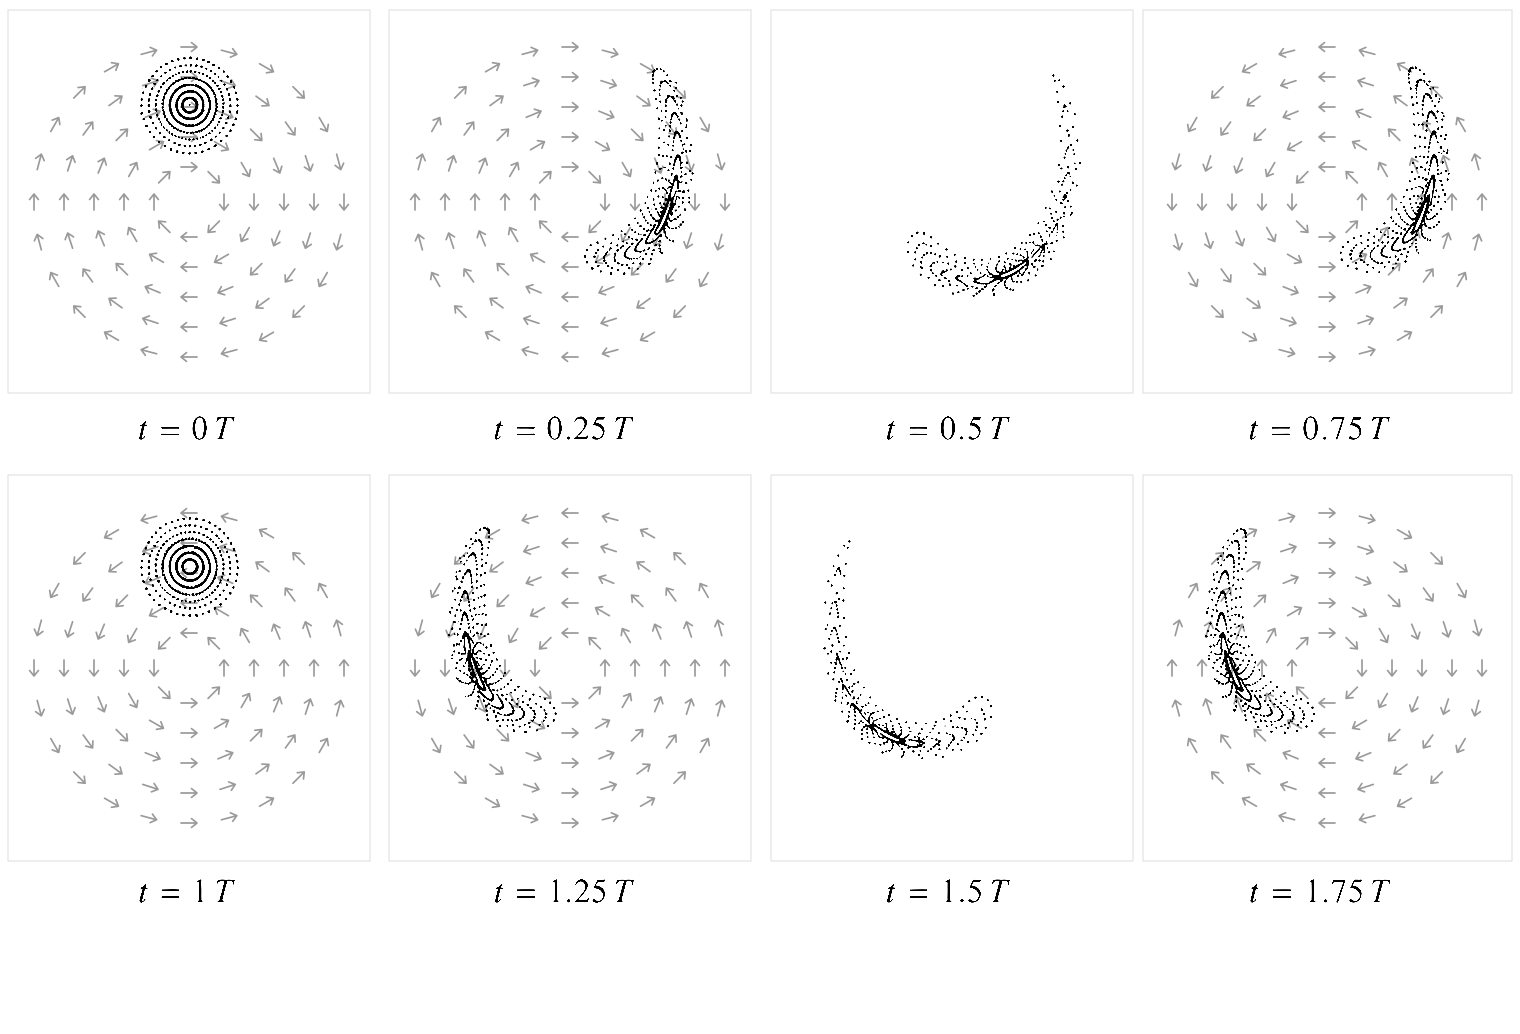
\includegraphics[width=0.9\linewidth,height=\textheight,keepaspectratio,alt={Rayleigh-Kothe particle sequence with velocity vectors}]{Images/CFDDEMCourse/tutorials-rayleigh-kothe-series-arrows.png}

The case-level \nolinkurl{precice-config.xml} defines the
\nolinkurl{Continuum} and \nolinkurl{Particles} participants, the
velocity data, their meshes, and a serial explicit coupling scheme.

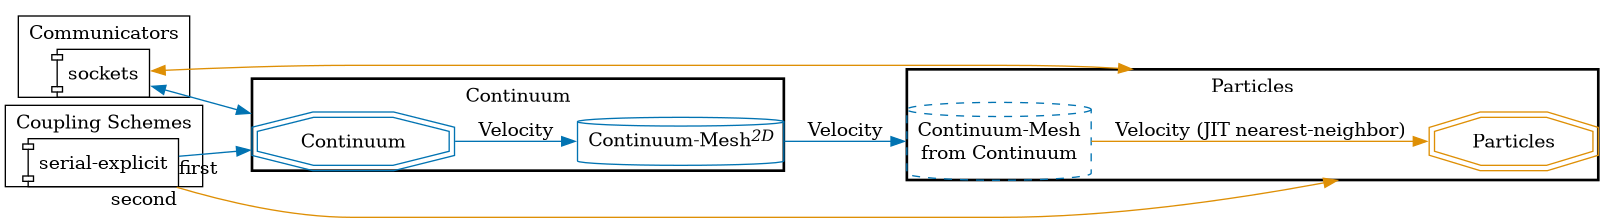
\includegraphics[width=0.9\linewidth,height=\textheight,keepaspectratio,alt={preCICE configuration visualization}]{Images/CFDDEMCourse/tutorials-rayleigh-kothe-precice-config.png}

\subsection{Step 3: Running the
Case}\label{01-rayleigh-kothe__readmemd__step-3-running-the-case}

Open two terminals in this case. Start the analytical participant in the
first:

\noindent\begin{minipage}{\linewidth}
\begin{Verbatim}[breaklines=true,breaksymbolleft={},breaksymbolright={},fontsize=\footnotesize]
cd "$SETUPS_ROOT/01-rayleigh-kothe/fluid-analytical"
source .venv/bin/activate
./run.sh
\end{Verbatim}
\end{minipage}

Start MercuryDPM in the second:

\noindent\begin{minipage}{\linewidth}
\begin{Verbatim}[breaklines=true,breaksymbolleft={},breaksymbolright={},fontsize=\footnotesize]
cd "$SETUPS_ROOT/01-rayleigh-kothe/particles-mercurydpm"
./run.sh --build-dir="$MERCURYDPM_BUILD_DIR"
\end{Verbatim}
\end{minipage}

It is normal for the first participant to wait until the second one
starts. Use the participant-local \nolinkurl{clean.sh} scripts before
repeating a run.

\subsection{Step 4: Inspecting the
Result}\label{01-rayleigh-kothe__readmemd__step-4-inspecting-the-result}

Open the generated \nolinkurl{RayleighKotheParticle_*.vtu} sequence in
ParaView. Over one coupling period, the particles should deform with the
vortex and then return close to their starting positions.

\subsubsection{Optional accuracy task: compare two
mappings}\label{01-rayleigh-kothe__readmemd__optional-accuracy-task-compare-two-mappings}

The supplied configuration uses nearest-neighbor mapping. This is a
computationally cheap and robust choice, but it assigns the value of the
closest continuum vertex and therefore produces a piecewise-constant
approximation of the analytical velocity field.

First run the case with the supplied configuration. Then replace the
\nolinkurl{mapping:nearest-neighbor} XML tag in the
\nolinkurl{Particles} participant (line 30 in the
\nolinkurl{precice-config.xml}) with a partition-of-unity RBF mapping
using a compact polynomial C6 basis function:

\noindent\begin{minipage}{\linewidth}
\begin{Verbatim}[breaklines=true,breaksymbolleft={},breaksymbolright={},fontsize=\footnotesize]
<mapping:rbf-pum-direct
  direction="read"
  from="Continuum-Mesh"
  constraint="consistent"
  project-to-input="false">
  <basis-function:compact-polynomial-c6 support-radius="2" />
</mapping:rbf-pum-direct>
\end{Verbatim}
\end{minipage}

Clean and rerun both participants, then compare the initial and final
particle positions in ParaView. After one vortex period, do the
particles reach their exact starting positions? You may also change the
\nolinkurl{110}-by-\nolinkurl{110} continuum mesh resolution, e.g.,
reduce \nolinkurl{num_vertices_x} and \nolinkurl{num_vertices_y} in
\nolinkurl{fluid-analytical/rayleigh-kothe-function.py}, use the same
resolution for both mappings, and repeat the comparison.

\section[Channel particle transport]{Case 2: Channel transport with OpenFOAM and MercuryDPM}\label{02-channel-transport-particles__readmemd__case-2-channel-transport-with-openfoam-and-mercurydpm}

This case replaces the analytical flow field from case 1 with a
two-dimensional incompressible CFD simulation. OpenFOAM computes flow
through a channel with an obstacle and sends velocity to MercuryDPM. The
particles remain passive: they do not affect the fluid.

The setup follows the preCICE
\href{https://precice.org/tutorials-channel-transport-particles}{channel
transport with particles tutorial}.

\subsection{Step 1: Compiling Software: OpenFOAM and Its preCICE
Adapter}\label{02-channel-transport-particles__readmemd__step-1-compiling-software-openfoam-and-its-precice-adapter}

This case reuses \nolinkurl{COURSE_ROOT}, \nolinkurl{SETUPS_ROOT},
\nolinkurl{PRECICE_ROOT}, \nolinkurl{MERCURYDPM_BUILD_DIR}, and the
preCICE search paths configured in case 1. Make sure that persistent
environment is loaded in each new terminal.

Keep the preCICE and MercuryDPM installations from case 1; its build
step already created \nolinkurl{ChannelTransport}. Follow the preCICE
guide on
\href{https://precice.org/adapter-openfoam-support.html\#how-to-get-openfoam}{how
to get OpenFOAM} for installation options. Activate the OpenFOAM
environment in every terminal that builds or runs OpenFOAM. The supplied
material is known to work with OpenFOAM v2406, v2412, and v2512. For an
OpenFOAM v2512 package installation, the activation commands are
typically:

\noindent\begin{minipage}{\linewidth}
\begin{Verbatim}[breaklines=true,breaksymbolleft={},breaksymbolright={},fontsize=\footnotesize]
export OPENFOAM_BASHRC=/usr/lib/openfoam/openfoam2512/etc/bashrc
source "$OPENFOAM_BASHRC"
\end{Verbatim}
\end{minipage}

Adjust only the assigned path for your installation, then use this same
variable in every OpenFOAM terminal. You can add both lines to
\nolinkurl{~/.bashrc}, or repeat them whenever you open a terminal.
Ensure that the \nolinkurl{PKG_CONFIG_PATH} and
\nolinkurl{LD_LIBRARY_PATH} settings for the preCICE installation from
case 1 are also active.

Extract and compile the bundled adapter after both OpenFOAM and preCICE
are available:

\noindent\begin{minipage}{\linewidth}
\begin{Verbatim}[breaklines=true,breaksymbolleft={},breaksymbolright={},fontsize=\footnotesize]
cd "$COURSE_ROOT/software"
tar -xzf openfoam-adapter-dev.tar.gz
cd openfoam-adapter-dev
./Allwmake
foamHasLibrary -verbose precice libpreciceAdapterFunctionObject
\end{Verbatim}
\end{minipage}

The final command should report that both libraries can be loaded. If
compilation fails, inspect \nolinkurl{wmake.log} and \nolinkurl{ldd.log}
in the adapter directory.

\subsection{Step 2: Understanding the Setup and
Configuration}\label{02-channel-transport-particles__readmemd__step-2-understanding-the-setup-and-configuration}

Particles start as a compact circular cloud near the inlet. The fluid
flows from left to right around the obstacle and transports the cloud
downstream.

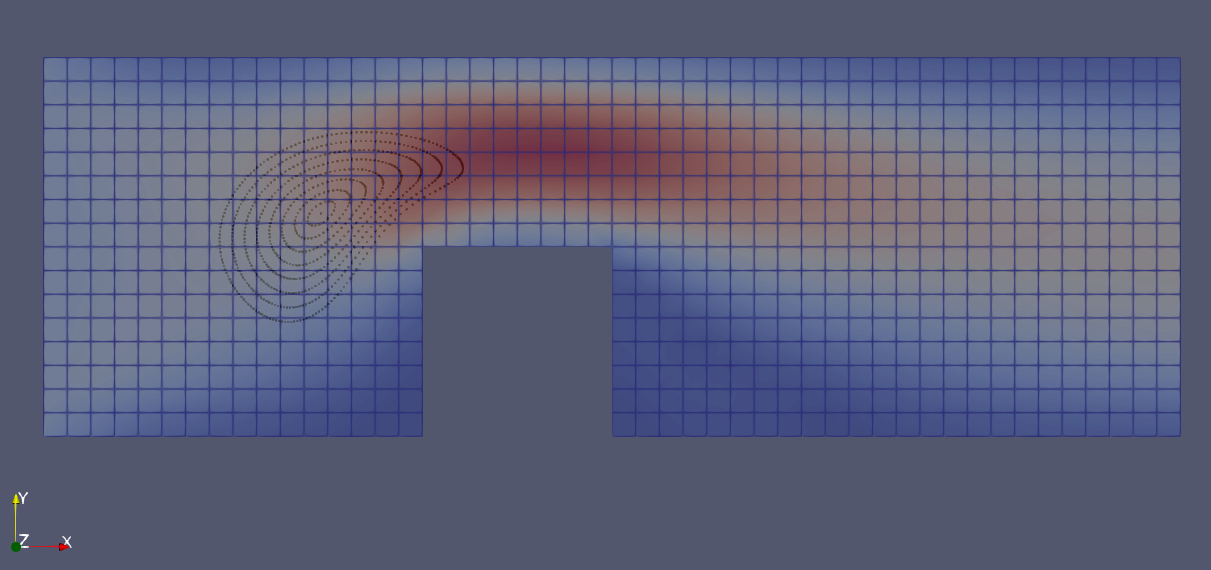
\includegraphics[width=0.9\linewidth,height=\textheight,keepaspectratio,alt={Channel transport setup}]{Images/CFDDEMCourse/tutorials-channel-transport-particles-setup.png}

The OpenFOAM adapter is configured in
\nolinkurl{fluid-openfoam/system/preciceDict}. The case-level
\nolinkurl{precice-config.xml} couples \nolinkurl{Fluid} to
\nolinkurl{Particles}, exchanges velocity in one direction, and maps it
to particle positions just in time.

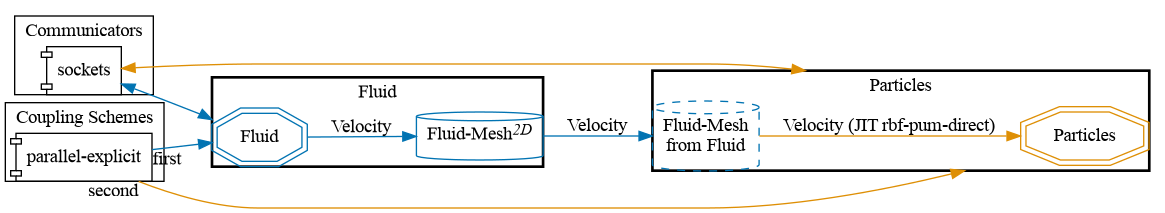
\includegraphics[width=0.9\linewidth,height=\textheight,keepaspectratio,alt={preCICE configuration visualization}]{Images/CFDDEMCourse/tutorials-channel-transport-particles-precice-config.png}

\subsection{Step 3: Running the
Case}\label{02-channel-transport-particles__readmemd__step-3-running-the-case}

Activate OpenFOAM and start the fluid participant in the first terminal:

\noindent\begin{minipage}{\linewidth}
\begin{Verbatim}[breaklines=true,breaksymbolleft={},breaksymbolright={},fontsize=\footnotesize]
source "$OPENFOAM_BASHRC"
cd "$SETUPS_ROOT/02-channel-transport-particles/fluid-openfoam"
./run.sh
\end{Verbatim}
\end{minipage}

Start the particle participant in the second terminal:

\noindent\begin{minipage}{\linewidth}
\begin{Verbatim}[breaklines=true,breaksymbolleft={},breaksymbolright={},fontsize=\footnotesize]
cd "$SETUPS_ROOT/02-channel-transport-particles/particles-mercurydpm"
./run.sh --build-dir="$MERCURYDPM_BUILD_DIR"
\end{Verbatim}
\end{minipage}

Use the participant-local \nolinkurl{clean.sh} scripts before repeating
a run.

\subsection{Alternative: Using Nutils Instead of
OpenFOAM}\label{02-channel-transport-particles__readmemd__alternative-using-nutils-instead-of-openfoam}

Nutils provides a lightweight Python alternative to OpenFOAM; see the
\href{https://precice.org/adapter-nutils.html}{preCICE Nutils adapter
documentation} and the same
\href{https://precice.org/tutorials-channel-transport-particles}{channel
transport tutorial}. Start \nolinkurl{fluid-nutils/run.sh} instead of
\nolinkurl{fluid-openfoam/run.sh}, then run the unchanged MercuryDPM
participant from Step 3. The Nutils launcher creates a local virtual
environment and installs its Python requirements automatically. Note
that if you choose Nutils here, OpenFOAM is required for the
fluidized-bed case in case 3.

\noindent\begin{minipage}{\linewidth}
\begin{Verbatim}[breaklines=true,breaksymbolleft={},breaksymbolright={},fontsize=\footnotesize]
cd "$SETUPS_ROOT/02-channel-transport-particles/fluid-nutils"
./run.sh
\end{Verbatim}
\end{minipage}

\subsection{Step 4: Inspecting the
Result}\label{02-channel-transport-particles__readmemd__step-4-inspecting-the-result}

Open the generated fluid and particle VTK files in ParaView. Compare the
particle paths around the obstacle with the velocity field.

\section[Bidirectional fluidized-bed coupling]{Case 3: Bidirectional CFD--DEM coupling in a fluidized bed}\label{03-link-fluidized-bed__readmemd__case-3-bidirectional-cfd-dem-coupling-in-a-fluidized-bed}

The final case reproduces Case A from J. M. Link, L. A. Cuypers, N. G.
Deen, and J. A. M. Kuipers, ``Flow regimes in a spout-fluid bed: a
combined experimental and simulation study,'' \emph{Chemical Engineering
Science} 60(13) (2005), 3425--3442,
\href{https://doi.org/10.1016/j.ces.2005.01.027}{doi:10.1016/j.ces.2005.01.027}.
The case and further methodological details are documented in D.
Schneider, \emph{Flexible and Efficient Data Mapping for Simulation of
Coupled Problems}, PhD thesis, Universität Stuttgart, 2026,
\href{https://doi.org/10.18419/opus-18423}{doi:10.18419/opus-18423}. The
setup and data provided here were largely adopted from D. Schneider,
\emph{Replication Data for: A Modular Approach for Mesh-Particle
Coupling}, DaRUS, 2025,
\href{https://doi.org/10.18419/DARUS-5494}{doi:10.18419/DARUS-5494}.

OpenFOAM solves the volume-averaged Navier--Stokes equations and
MercuryDPM resolves the particles. Fluid velocity and pressure gradient
drive the particles, while particle volume fraction and momentum
exchange feed back into the fluid.

\subsection{Step 1: Compiling Software: Custom OpenFOAM and MercuryDPM
Solvers}\label{03-link-fluidized-bed__readmemd__step-1-compiling-software-custom-openfoam-and-mercurydpm-solvers}

This case reuses the persistent course environment from case 1 and the
OpenFOAM activation path from case 2. Make sure both are loaded in each
new terminal.

Keep preCICE, MercuryDPM, OpenFOAM, and the OpenFOAM adapter from the
previous cases. The MercuryDPM build from case 1 already contains
\nolinkurl{SettleFluidizedBed} and \nolinkurl{FluidizedBed}.

Activate OpenFOAM, extract the custom solver, and compile it with
\nolinkurl{wmake}:

\noindent\begin{minipage}{\linewidth}
\begin{Verbatim}[breaklines=true,breaksymbolleft={},breaksymbolright={},fontsize=\footnotesize]
source "$OPENFOAM_BASHRC"
cd "$COURSE_ROOT/software"
tar -xzf openfoam-solver.tar.gz
cd openfoam-solver
wmake
command -v AndersonJacksonFoam
\end{Verbatim}
\end{minipage}

The final command should locate \nolinkurl{AndersonJacksonFoam},
normally under \nolinkurl{$FOAM_USER_APPBIN}. If
\nolinkurl{OPENFOAM_BASHRC} is empty, configure it as described in case
2 and use the same value in every OpenFOAM terminal.

\subsection{Step 2: Understanding the Setup and
Configuration}\label{03-link-fluidized-bed__readmemd__step-2-understanding-the-setup-and-configuration}

The domain is a narrow fluidized bed with a packed particle layer and an
upward gas flow. \nolinkurl{fluid-openfoam/} contains the CFD case,
while \nolinkurl{particles-mercurydpm/} contains the DEM launcher and a
prepared settling restart archive.

Before the first run, unpack the initial particle state:

\noindent\begin{minipage}{\linewidth}
\begin{Verbatim}[breaklines=true,breaksymbolleft={},breaksymbolright={},fontsize=\footnotesize]
cd "$SETUPS_ROOT/03-link-fluidized-bed/particles-mercurydpm"
tar -xzf settled-restart-file.tar.gz
\end{Verbatim}
\end{minipage}

The OpenFOAM adapter configuration is in
\nolinkurl{fluid-openfoam/system/preciceDict}. The case-level
\nolinkurl{precice-config.xml} exchanges velocity, pressure gradient,
solid volume fraction, and explicit and implicit momentum terms using a
serial explicit scheme and just-in-time mappings.

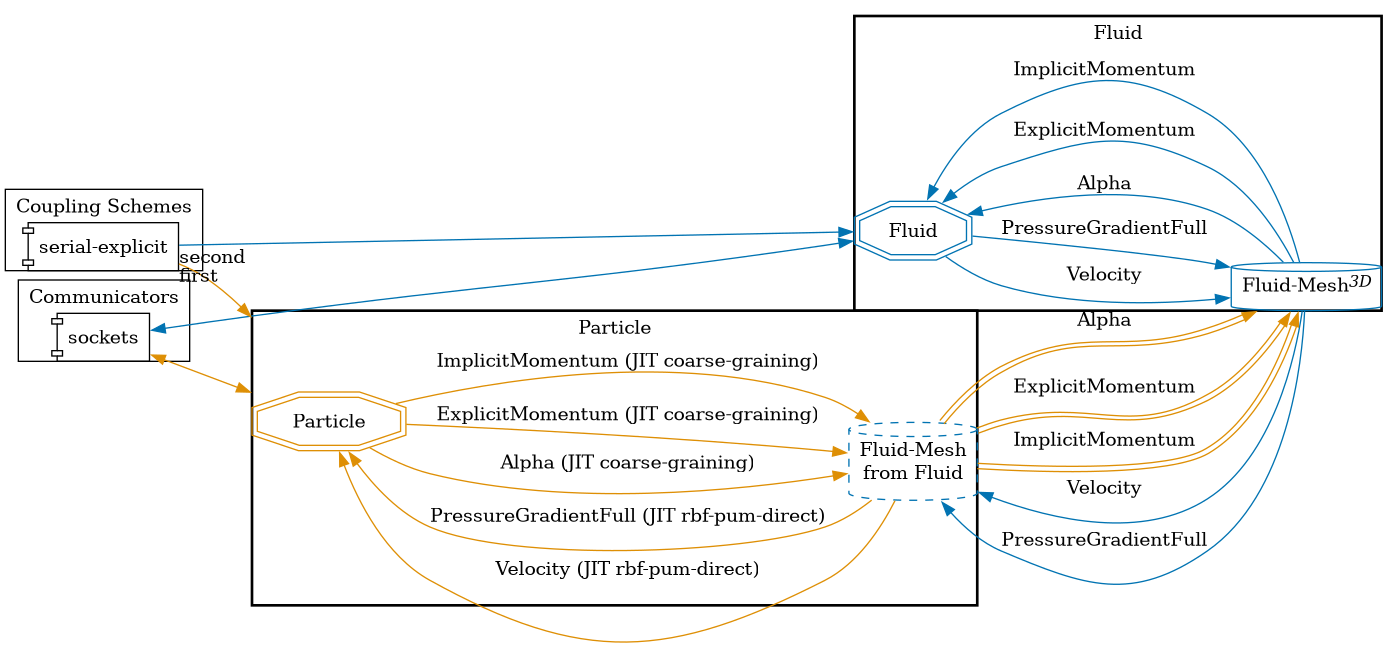
\includegraphics[width=0.9\linewidth,height=\textheight,keepaspectratio,alt={preCICE configuration visualization}]{Images/CFDDEMCourse/tutorials-link-fluidized-bed-precice-config.png}

\subsection{Step 3: Running the
Case}\label{03-link-fluidized-bed__readmemd__step-3-running-the-case}

Activate OpenFOAM and start the fluid participant in the first terminal:

\noindent\begin{minipage}{\linewidth}
\begin{Verbatim}[breaklines=true,breaksymbolleft={},breaksymbolright={},fontsize=\footnotesize]
source "$OPENFOAM_BASHRC"
cd "$SETUPS_ROOT/03-link-fluidized-bed/fluid-openfoam"
./run.sh
\end{Verbatim}
\end{minipage}

Start the MercuryDPM participant in the second terminal:

\noindent\begin{minipage}{\linewidth}
\begin{Verbatim}[breaklines=true,breaksymbolleft={},breaksymbolright={},fontsize=\footnotesize]
cd "$SETUPS_ROOT/03-link-fluidized-bed/particles-mercurydpm"
./run.sh --build-dir="$MERCURYDPM_BUILD_DIR"
\end{Verbatim}
\end{minipage}

The particle launcher runs \nolinkurl{FluidizedBed} with six OpenMP
threads. The prepared restart avoids recomputing the settling;
\nolinkurl{SettleFluidizedBed} is available if you want to regenerate
it. Clean both participant directories before repeating an interrupted
run.

\subsection{Alternative: Using LIGGGHTS Instead of
MercuryDPM}\label{03-link-fluidized-bed__readmemd__alternative-using-liggghts-instead-of-mercurydpm}

The course bundle also contains a modified LIGGGHTS version with the
preCICE coupling and pressure-gradient exchange required by this case.
It needs MPI and \href{https://github.com/chr1shr/voro}{Voro++}. On
Ubuntu, install the library and its development files with:

\noindent\begin{minipage}{\linewidth}
\begin{Verbatim}[breaklines=true,breaksymbolleft={},breaksymbolright={},fontsize=\footnotesize]
sudo apt install voro++ voro++-dev
\end{Verbatim}
\end{minipage}

Alternatively, build Voro++ from source. The library must be compiled as
position-independent code so that LIGGGHTS can link it into its shared
library:

\noindent\begin{minipage}{\linewidth}
\begin{Verbatim}[breaklines=true,breaksymbolleft={},breaksymbolright={},fontsize=\footnotesize]
cd "$COURSE_ROOT/software"
git clone https://github.com/chr1shr/voro.git
cd voro
mkdir -p build
cd build
export VORO_ROOT="$COURSE_ROOT/software/voro-install"
cmake \
  -DCMAKE_BUILD_TYPE=Release \
  -DCMAKE_POSITION_INDEPENDENT_CODE=ON \
  -DCMAKE_INSTALL_PREFIX="$VORO_ROOT" \
  ..
make -j4
make install
export CMAKE_PREFIX_PATH="$VORO_ROOT${CMAKE_PREFIX_PATH:+:$CMAKE_PREFIX_PATH}"
\end{Verbatim}
\end{minipage}

With Voro++ installed and preCICE discoverable in the current
environment, build LIGGGHTS from the bundle\textquotesingle s
\nolinkurl{software/} directory:

\noindent\begin{minipage}{\linewidth}
\begin{Verbatim}[breaklines=true,breaksymbolleft={},breaksymbolright={},fontsize=\footnotesize]
cd "$COURSE_ROOT/software"
tar -xzf liggghts-dev.tar.gz
cd liggghts-dev
mkdir -p build
cd build
export LIGGGHTS_ROOT="$COURSE_ROOT/software/liggghts-install"
cmake \
  -DCMAKE_INSTALL_PREFIX="$LIGGGHTS_ROOT" \
  -DCMAKE_BUILD_TYPE=Release \
  -DENABLE_PRECICE=ON \
  -DENABLE_MODEL_HOOKE_STIFFNESS=ON \
  -DENABLE_MODEL_TANGENTIAL_HISTORY=ON \
  -DENABLE_MODEL_COHESION_OFF=ON \
  -DENABLE_MODEL_ROLLING_OFF=ON \
  -DENABLE_MODEL_SURFACE_DEFAULT=ON \
  -DENABLE_MPI=ON \
  -DENABLE_VORONOI=ON \
  -DENABLE_VTK=ON \
  ../src
make -j4
make install
export PATH="$LIGGGHTS_ROOT/bin:$PATH"
\end{Verbatim}
\end{minipage}

As in case 1, the optional Voro++ and LIGGGHTS exports must be set in
every terminal that builds or runs LIGGGHTS. Add \nolinkurl{VORO_ROOT},
\nolinkurl{LIGGGHTS_ROOT}, the updated \nolinkurl{CMAKE_PREFIX_PATH},
and \nolinkurl{PATH} commands to \nolinkurl{~/.bashrc} if you want to
keep them across terminals.

Keep the OpenFOAM participant from Step 3. In the particle terminal, use
the LIGGGHTS case instead:

\noindent\begin{minipage}{\linewidth}
\begin{Verbatim}[breaklines=true,breaksymbolleft={},breaksymbolright={},fontsize=\footnotesize]
cd "$SETUPS_ROOT/03-link-fluidized-bed/particles-liggghts"
tar -xzf settled-restart-file.tar.gz
./run.sh
\end{Verbatim}
\end{minipage}

This launches two MPI ranks using \nolinkurl{in.cfdem.liggghts}. The
commented command in \nolinkurl{run.sh} shows how to regenerate the
settled state. Clean the OpenFOAM and LIGGGHTS directories before
switching particle solvers or restarting a run.

The coupling commands are in \nolinkurl{in.cfdem.liggghts}. If you
change the preCICE mapping radius, keep the mirror width in the
\nolinkurl{fluid_coupling} command consistent with it (both are
\nolinkurl{0.008} in the supplied case). The
\nolinkurl{precice_initialize} command also specifies a
\nolinkurl{0.015} safety margin around the fluid mesh; revisit it if the
geometry or mapping support changes.

\subsection{Step 4: Inspecting and Comparing the
Result}\label{03-link-fluidized-bed__readmemd__step-4-inspecting-and-comparing-the-result}

Open the OpenFOAM fields and the MercuryDPM or LIGGGHTS VTK snapshots in
ParaView. The supplied result archives provide reference runs. The
\nolinkurl{postprocessing/} directory contains the Link et al. reference
data, processed MercuryDPM and LIGGGHTS results, plotting scripts, and
\nolinkurl{comparison-all.pdf} for a compact quantitative comparison.

\subsection{Advanced Topic: Postprocessing and Solver
Comparison}\label{03-link-fluidized-bed__readmemd__advanced-topic-postprocessing-and-solver-comparison}

The comparison evaluates the vertical particle mass flux across the bed.
To coarse-grain a completed MercuryDPM run, execute
\nolinkurl{MercuryCG} from the case root, replacing the input name or
time interval if your run differs:

\noindent\begin{minipage}{\linewidth}
\begin{Verbatim}[breaklines=true,breaksymbolleft={},breaksymbolright={},fontsize=\footnotesize]
cd "$SETUPS_ROOT/03-link-fluidized-bed"
"$MERCURYDPM_BUILD_DIR/Drivers/MercuryCG/MercuryCG" FluidizedBed \
  -coordinates XY -x -0.075 0.075 -y 0.125 0.135 -ny 1 -nx 40 \
  -timeaverage -tmin 2.5 -tmax 6 -function Lucy -w 0.005 \
  -o postprocessing/mercury-1-5s-to-5s-w0-005-x40.dat
\end{Verbatim}
\end{minipage}

For LIGGGHTS, unpack the averaged raw data and convert it to the common
profile format:

\noindent\begin{minipage}{\linewidth}
\begin{Verbatim}[breaklines=true,breaksymbolleft={},breaksymbolright={},fontsize=\footnotesize]
cd "$SETUPS_ROOT/03-link-fluidized-bed/postprocessing"
tar -xzf liggghts-averaged-data.tar.gz
python3 process-liggghts-averaged-data.py \
  --file liggghts-results-1-5-to-5.dat --dx 0.00375 --dy 0.01
\end{Verbatim}
\end{minipage}

By default, the script uses the last available timestamp and writes its
files under \nolinkurl{liggghts-results/}. Use \nolinkurl{--time <N>} to
select another cumulative average. The supplied
\nolinkurl{liggghts-1-5s-to-5s-x40.csv} is the already processed profile
from the reference run and is used in the command below.

Finally, compare both particle solvers with the Link et al. experimental
data and Koch-Hill result:

\noindent\begin{minipage}{\linewidth}
\begin{Verbatim}[breaklines=true,breaksymbolleft={},breaksymbolright={},fontsize=\footnotesize]
python3 plot-comparison-all.py \
  --ref Link2005.dat \
  --mercury mercury-1-5s-to-5s-w0-005-x40.dat \
  --liggghts liggghts-1-5s-to-5s-x40.csv \
  --pdf comparison-all.pdf
\end{Verbatim}
\end{minipage}

The generated MercuryDPM particle data can be large. The processed
profiles and \nolinkurl{comparison-all.pdf} are therefore already
included, so this advanced step can also be studied without rerunning or
retaining every raw output file.
